%! TeX root = openfoam_presentation.tex
\usetheme[framenumber-footline]{Mumbai}



\usepackage[edges]{forest}
\usepackage{siunitx}
\usepackage{tikz}
\usetikzlibrary{3d, perspective}
\usepackage{xparse}



\def\blockmesh{\texttt{blockMesh}}
\def\lapfoam{\texttt{laplacianFoam}}
\def\openfoam{\texttt{OpenFOAM}}
\def\paraview{\texttt{ParaView}}
\def\parafoam{\texttt{paraFoam}}
\NewDocumentCommand{\pder}{omm}{%
    \IfNoValueTF{#1}{\ensuremath{\frac{\partial #2}{\partial #3}}}{\ensuremath{\frac{\partial^#1 #2}{\partial #3^#1}}}
}
%\newcommand{\pder}[2]{\ensuremath{\frac{\partial #1}{\partial #2}}}
\newcommand{\setitemsep}[1]{\setlength\itemsep{#1}}




\begin{document}

\title{Introduction to \openfoam}
\author{Vachan Potluri}
\date{April 2023}

{
\setbeamertemplate{footline}{}
\frame{\maketitle}
}

\begin{frame}
    \begin{block}{What}
        \begin{itemize}
            \item CFD software (but without GUI)
            \item \textbf{Open} source \textbf{F}ield \textbf{O}peration \textbf{A}nd \textbf{M}anipulation
            \item Open source $\implies$ source code is given to user
        \end{itemize}
    \end{block}
\onslide<2->
    \begin{figure}
        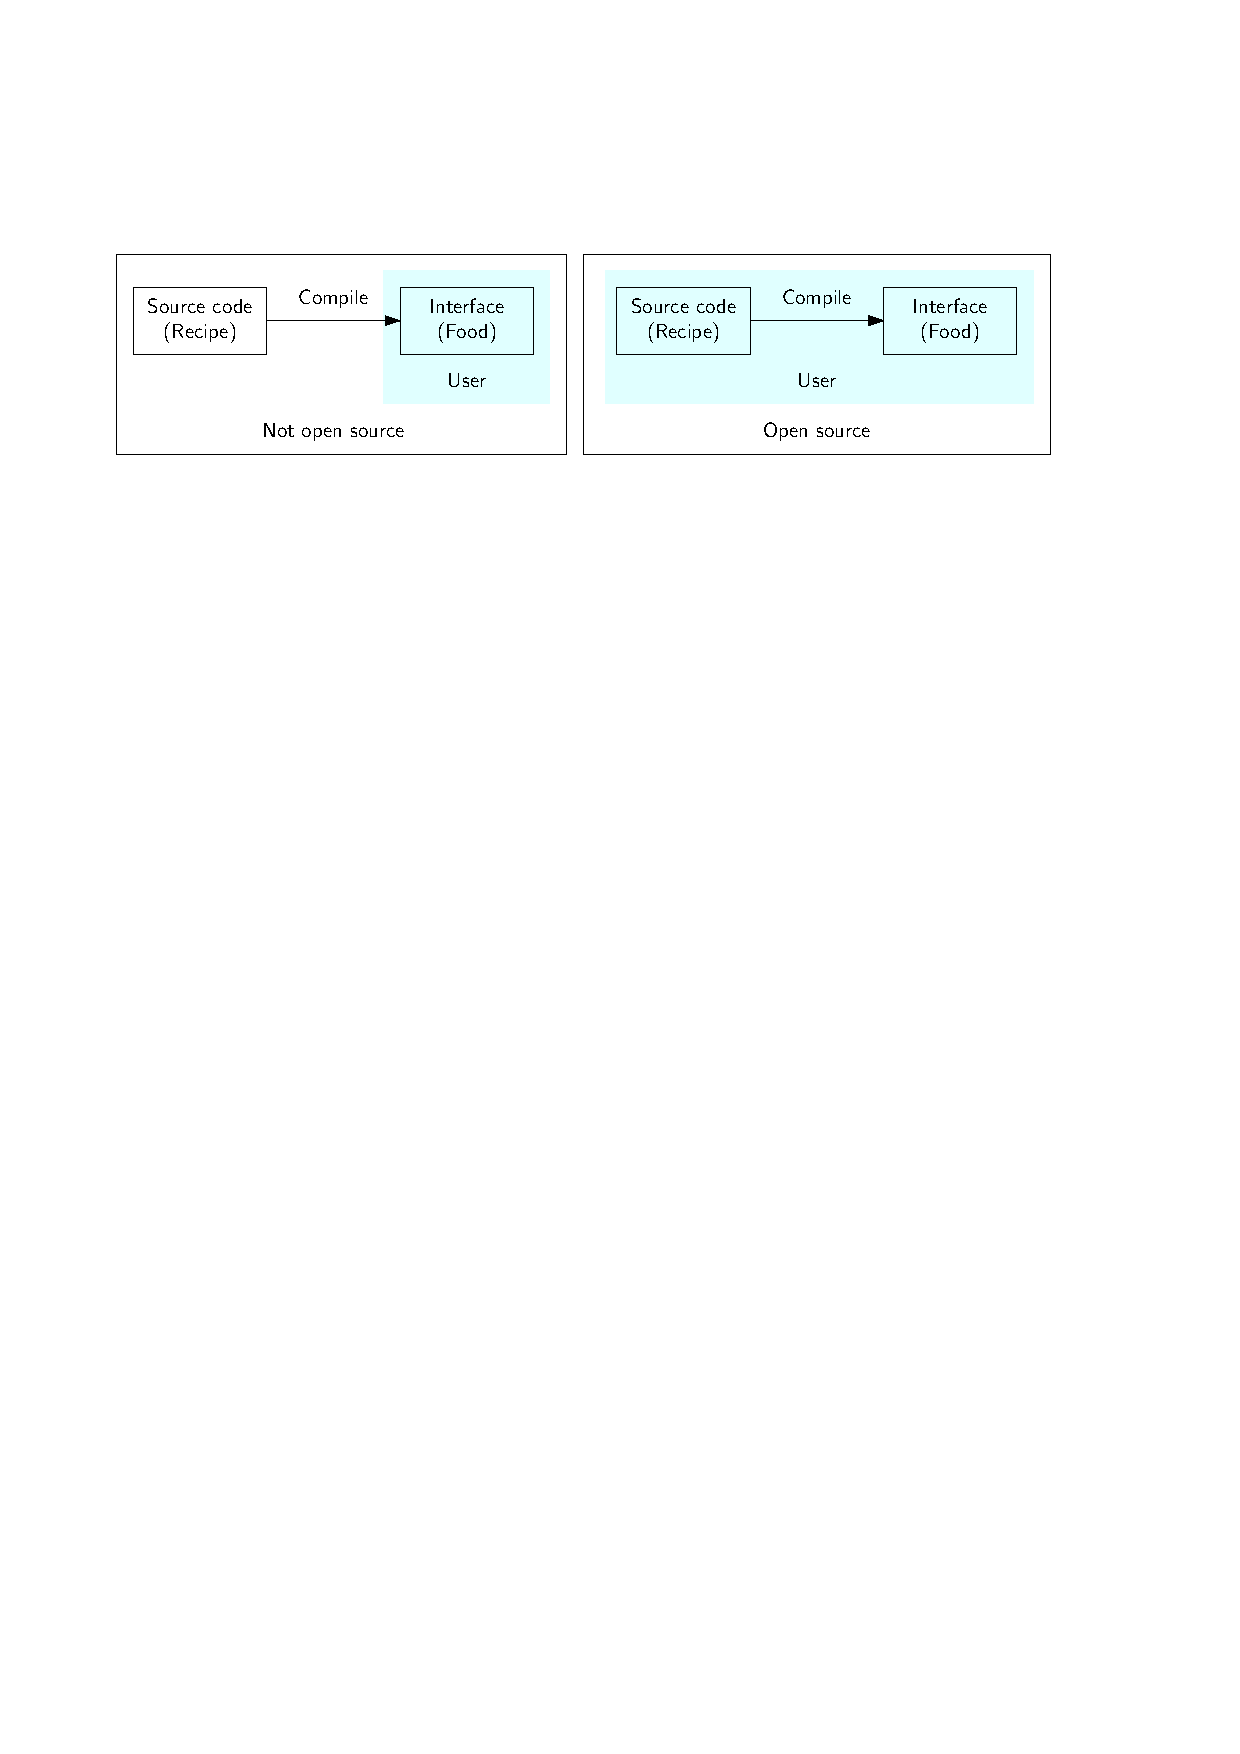
\includegraphics[width=\linewidth]{opensource_illustration}
    \end{figure}
\onslide<3->
    No GUI $\implies$ hard to learn
    \begin{block}{Why}
        \begin{itemize}
            \item Free
            \item Fast
            \item User customisable: solve any equation you desire
        \end{itemize}
    \end{block}
\end{frame}

\begin{frame}{Case 1}{Heat conduction in a square plate}
    \begin{columns}
        \begin{column}{0.5\linewidth}
            \begin{equation*}
                \pder{T}{t} = D_T \left( \pder[2]{T}{x} + \pder[2]{T}{y} \right)
            \end{equation*}
            \begin{figure}
                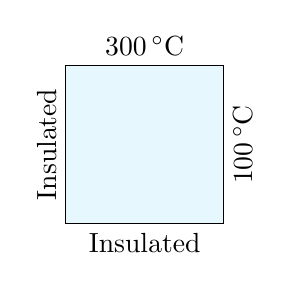
\begin{tikzpicture}[scale=2]
                    \draw [fill=cyan!10] (0,0) -- node [below] {Insulated} (1,0) -- node [rotate=90, below] {\qty{100}{\degreeCelsius}} (1,1) -- node [above] {\qty{300}{\degreeCelsius}} (0,1) -- node [rotate=90, above] {Insulated} cycle;
                \end{tikzpicture}
            \end{figure}
        \end{column}
        \begin{column}{0.5\linewidth}
            Other settings
            \begin{itemize}
                \item $D_T=\qty{1}{m^2/s}$
                \item $L=\qty{1}{m}$
                \item End time \qty{5}{s}
            \end{itemize}
        \end{column}
    \end{columns}
\onslide<2->
    \begin{itemize}
        \item \lapfoam{} is the ``solver'' to be used for heat conduction equation
        \item Visualise using \parafoam
        \begin{itemize}
            \item Mesh representation
            \item Data array selection
            \item Navigating times
        \end{itemize}
    \end{itemize}
\end{frame}

\begin{frame}{\openfoam's simulation setup}
    \begin{columns}
        \begin{column}{0.5\linewidth}
            \begin{block}{Case structure for \lapfoam}
                \begin{figure}
                    \centering
                    \begin{forest}
                        for tree={
                            font=\ttfamily,
                            grow'=0,
                            child anchor=west,
                            parent anchor=south,
                            anchor=west,
                            calign=first,
                            edge path={
                                \noexpand\path [draw, \forestoption{edge}]
                                (!u.south west) +(7.5pt,0) |- node[circle,fill,inner sep=1.25pt] {} (.child anchor)\forestoption{edge label};
                            },
                            before typesetting nodes={
                                if n=1
                                {insert before={[,phantom]}}
                                {}
                            },
                            fit=band,
                            before computing xy={l=15pt},
                        }
                        [case\_name/
                            [0/
                                [T]
                            ]
                            [constant/
                                [physicalProperties]
                                [polyMesh/*]
                            ]
                            [system/
                                [controlDict]
                                [fvSchemes]
                                [fvSolution]
                            ]
                        ]
                    \end{forest}
                \end{figure}
            \end{block}
        \end{column}
        \begin{column}{0.5\linewidth}
            \begin{itemize}
                \setitemsep{1em}
                \item Every simulation is setup using certain ``setting'' files
                \item These files are grouped into 3 folders: \texttt{0/}, \texttt{constant/} and \texttt{system/}
                \item All are text files
\onslide<2->
                \item Only mandatory files are shown here, there can be additional files also
                \item When a simulation is done, \openfoam{} generates corresponding time files
                \item We will learn about these files by doing some variations of the square plate simulation
            \end{itemize}
        \end{column}
    \end{columns}
\end{frame}

\begin{frame}{Case 1, variation 1}{Change the thermal diffusivity}
    \begin{itemize}
        \setitemsep{1em}
        \item In \texttt{constant/physicalProperties}, you can change $D_T$
        \item Things to note
        \begin{itemize}
            \item \texttt{FoamFile} ``header''
            \item Units of $D_T$
        \end{itemize}
        \item Try
        \begin{itemize}
            \item Reduce $D_T$ to \qty{0.01}{m^2/s} and see the solution evolution
        \end{itemize}
        \item Tips
        \begin{itemize}
            \item \texttt{foamListTimes -rm} deletes all time folders other than \texttt{0/}
            \item Reload files in \paraview{} by right-clicking
        \end{itemize}
    \end{itemize}
\end{frame}

\begin{frame}{Case 1, variation 2}{Change the boundary conditions}
    \begin{itemize}
        \setitemsep{1em}
        \item In \texttt{0/T} you can set initial condition (IC) and boundary conditions (BCs)
        \item Things to note
        \begin{itemize}
            \item \texttt{internalField} $\implies$ IC
            \item Names of different boundaries
            \item \texttt{type} of different boundaries $\implies$ type of BC
        \end{itemize}
        \item Special BC type \texttt{empty}
        \begin{itemize}
            \item By default \openfoam{} does 3d simulations
            \begin{itemize}
                \item Check this in \paraview
            \end{itemize}
            \item \texttt{empty} BC in a direction tells \openfoam{} to not consider that direction
        \end{itemize}
        \item Try
        \begin{itemize}
            \item Change bottom BC to \qty{-100}{\degreeCelsius}
            \item Change IC
            \item Do a 1d simulation by setting top and bottom boundaries as \texttt{zeroGradient}
            \begin{itemize}
                \item Verify the solution using ``Plot Over Line'' in \paraview{} or \texttt{gradTx} value
            \end{itemize}
        \end{itemize}
    \end{itemize}
\end{frame}

\begin{frame}{Case 1, variation 3}{Change time settings}
    \begin{itemize}
        \setitemsep{1em}
        \item \texttt{system/controlDict} contains all the main controls of the simulation
        \item Things to note
        \begin{itemize}
            \item \texttt{startFrom}, \texttt{stopAt}
            \item \texttt{startTime}, \texttt{endTime}
            \item \texttt{deltaT}
            \item \texttt{writeControl}, \texttt{writeInterval}
        \end{itemize}
        \item For heat conduction equation
        \begin{itemize}
            \item ``Stable'' time step value ($\Delta t_s$) satisfies $D_T \dfrac{\Delta t_s}{\Delta x^2} < 1$
            \item To determine end time ($t_e$), compare it with diffusion time scale
            \begin{equation*}
                t_e \gg \frac{L^2}{D_T} \implies \text{Steady state reached}
            \end{equation*}
        \end{itemize}
        \item Try
        \begin{itemize}
            \item Increase $D_T$ to \qty{10}{m^2/s}
            \item For correct simulation, time step and end time also have to be changed
        \end{itemize}
    \end{itemize}
\end{frame}

\begin{frame}{Case 1, variation 4}{Change the mesh}
    \begin{itemize}
        \setitemsep{1em}
        \item Multiple ways to create mesh in \openfoam
        \begin{itemize}
            \item Create in a different software (e.g. ANSYS) and import to \openfoam
            \item Use \openfoam's tools to create mesh
        \end{itemize}
        \item \blockmesh{} is one such tool in \openfoam{} to create meshes
        \item \blockmesh{} reads an additional file \texttt{system/blockMeshDict} to create mesh
        \item \texttt{system/blockMeshDict} has 3 components
        \begin{enumerate}
            \item Specify points or vertices
            \item Create ``blocks'' using these vertices
            \item Define boundaries using the vertices
        \end{enumerate}
    \end{itemize}
\end{frame}

\begin{frame}
    \begin{itemize}
        \setitemsep{1em}
        \item \openfoam{} defines a local coordinate system (LCS) for every block
        \item Blocks are created using a list of points ordered in a specific way
        \begin{enumerate}
            \item Point 0 is the origin of (LCS)
            \item Line 0-1 is along $x_1$ direction
            \item Line 1-2 is along $x_2$ direction
            \item Points 0-3 define plane $x_3=0$
            \item Points 4-7 are obtained by translating points 0-3 in $x_3$ direction
        \end{enumerate}
    \end{itemize}
    \begin{figure}
        \centering
        One of these is wrong.\\[0.5em]
        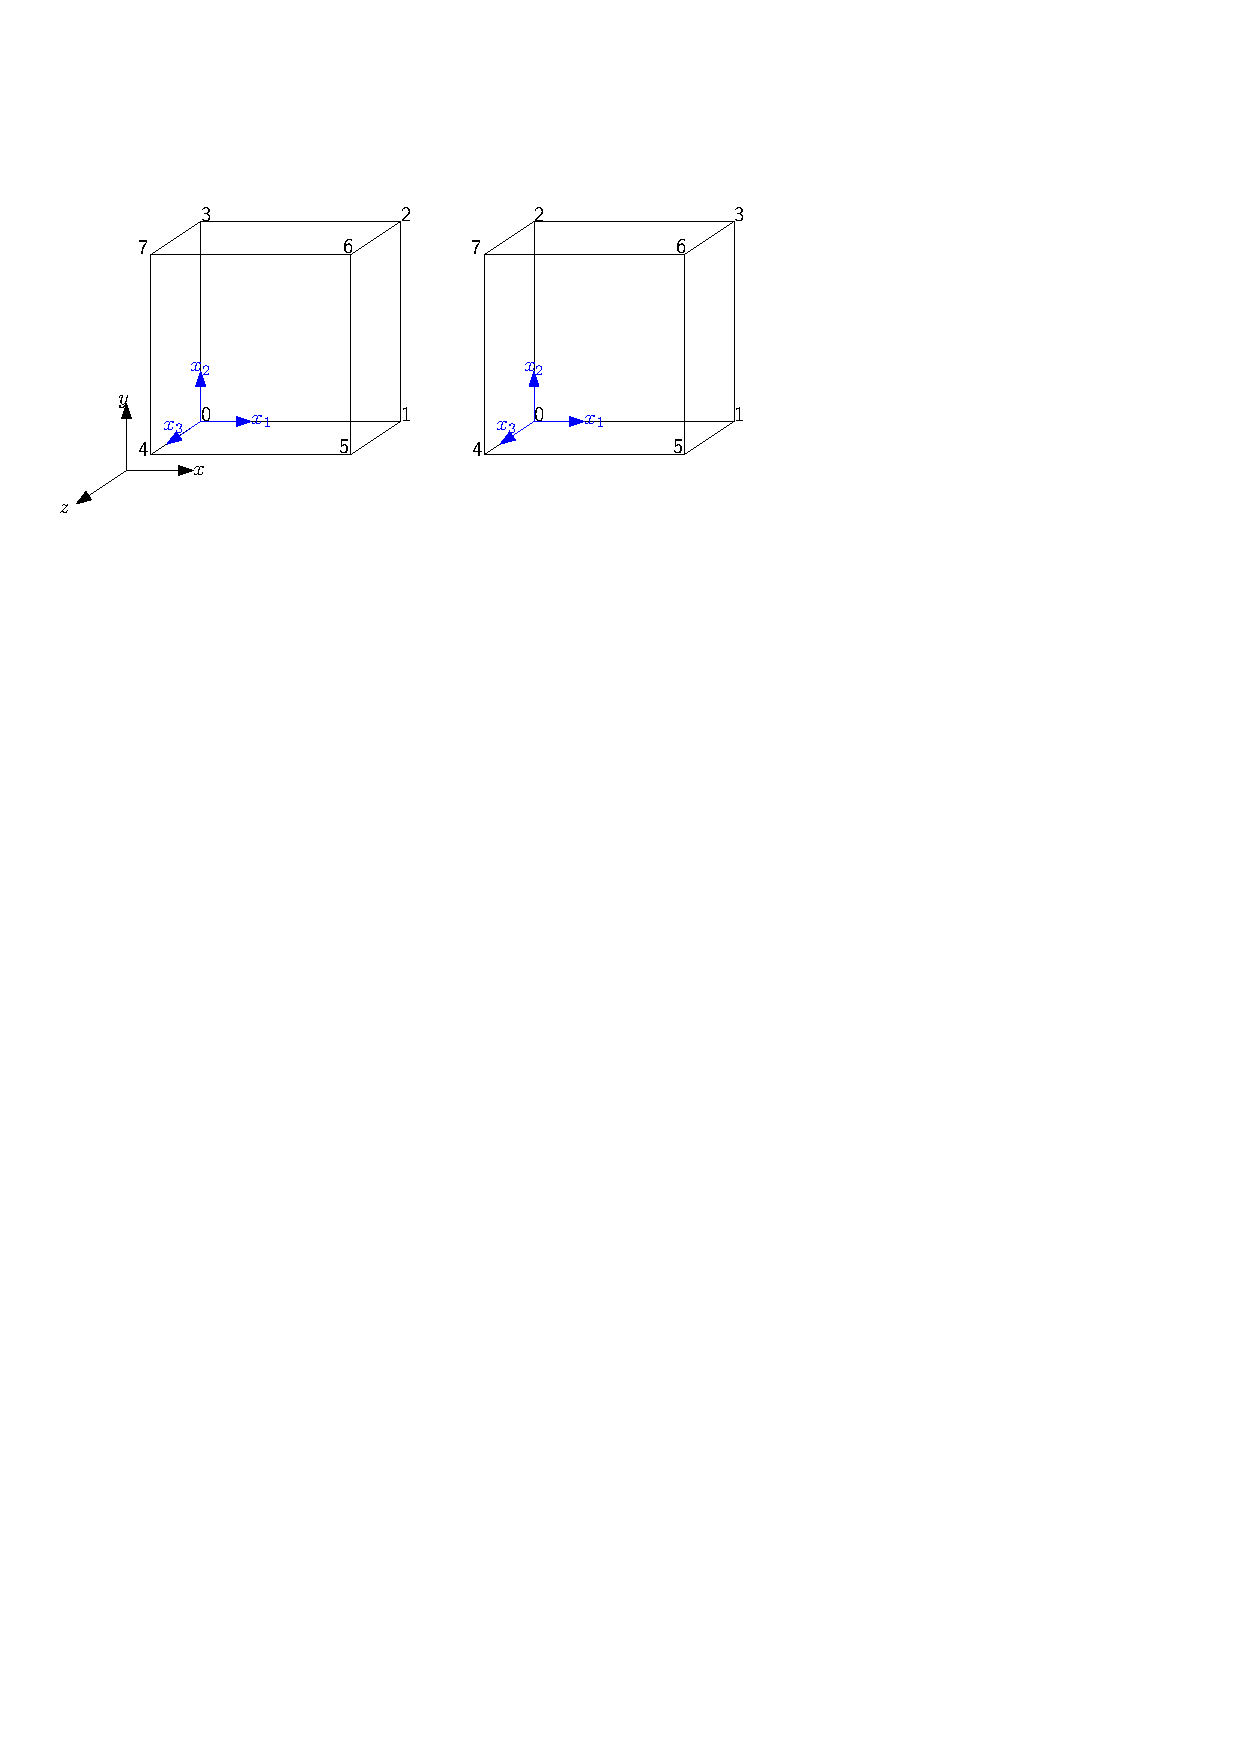
\includegraphics[width=0.8\linewidth]{blockmesh_ordering}
    \end{figure}
\end{frame}

\begin{frame}
    \begin{itemize}
        \setitemsep{1em}
        \item Boundaries are defined using a list of points such that right hand thumb rule points outward the block
        \item The boundary names in \texttt{system/blockMeshDict} and \texttt{0/T} must match
        \item Try
        \begin{itemize}
            \item Increasing mesh resolution
            \item Using mesh grading
            \item Changing geometry
        \end{itemize}
        \item Tips
        \begin{itemize}
            \item Run \texttt{blockMesh} command to update mesh
            \item Run \texttt{checkMesh} command to check if the mesh has no issues
            \item You can view different mesh regions (e.g. boundaries) individually in \paraview
        \end{itemize}
    \end{itemize}
\end{frame}

\begin{frame}{Case 2}{Heat conduction in an L-clamp}
    \begin{columns}
        \begin{column}{0.5\linewidth}
            \begin{figure}
                \centering
                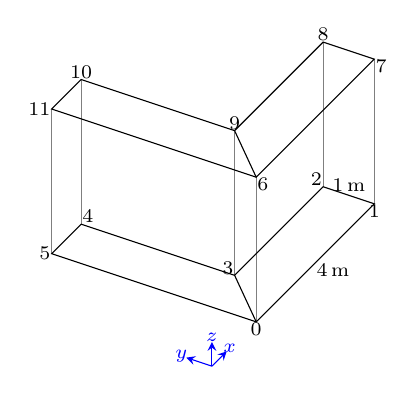
\begin{tikzpicture}[3d view={-60}{35.26}, >=stealth, inner sep=0.25pt, font=\scriptsize, scale=0.75]
                    \begin{scope}[shift={(-1.5,0,0)}, blue, scale=0.5]
                        \draw [->] (0,0,0) -- (1,0,0) node [pos=1.2] {$x$};
                        \draw [->] (0,0,0) -- (0,1,0) node [pos=1.2] {$y$};
                        \draw [->] (0,0,0) -- (0,0,1) node [pos=1.2] {$z$};
                    \end{scope}
                    
                    \begin{scope}[canvas is xy plane at z=0]
                        \draw (0,0) node [below] {0} -- node [anchor=north west] {\qty{4}{m}} (4,0) node [below] {1} -- node [above=1pt] {\qty{1}{m}} (4,1) node [anchor=south east] {2} -- (1,1) node [anchor=south east] {3} -- cycle;
                        \draw (1,1) -- (1,4) node [anchor=south west] {4} -- (0,4) node [left] {5} -- (0,0);
                    \end{scope}
                    
                    \begin{scope}[canvas is xy plane at z=3]
                        \draw (0,0) node [anchor=north west] {6} -- (4,0) node [anchor=north west] {7} -- (4,1) node [above] {8} -- (1,1) node [above] {9} -- cycle;
                        \draw (1,1) -- (1,4) node [above] {10} -- (0,4) node [left] {11} -- (0,0);
                    \end{scope}
                    
                    \foreach \p in {(0,0,0), (4,0,0), (4,1,0), (1,1,0), (0,4,0), (1,4,0)} {%
                        \draw [opacity=0.5] \p -- +(0,0,3);
                    }
                \end{tikzpicture}
            \end{figure}
            \begin{itemize}
                \item This geometry can be constructed using two blocks
                \begin{enumerate}
                    \item Block 1: (0 1 2 3 6 7 8 9)
                    \item Block 2: (0 3 4 5 6 9 10 11)
                \end{enumerate}
                \item Use single cell in $z$ direction and perpendicular to clamp
            \end{itemize}
        \end{column}
        \begin{column}{0.5\linewidth}
            \begin{itemize}
                \item Tip: you can see the mesh in \paraview{} without running the simulation
                \item BCs
                \begin{itemize}
                    \item One end (4 5 11 10) of clamp at \qty{100}{\degreeCelsius}
                    \item Other end (1 7 8 2) at \qty{0}{\degreeCelsius}
                    \item All other boundaries insulated
                    \item \texttt{empty} BC for top and bottom planes
                \end{itemize}
                \item Use $D_T=\qty{1}{m^2/s}$; set end time and time step accordingly
                \begin{gather*}
                    D_T \frac{\Delta t_s}{\Delta x} \le 1\\
                    t_e \gg \frac{L^2}{D_T}
                \end{gather*}
            \end{itemize}
        \end{column}
    \end{columns}
\end{frame}

\end{document}